\newcommand{\ppi}{Protein-Protein Interactions (PPI)}
\newcommand{\p}{Protein}

This chapter presents a brief summary on protein complexes, protein-protein 
interaction networks and the current state of protein-protein interaction network 
analysis and talks about other similar work that has been done in this area. 
Naturally, this chapter will be consistently updated as we make further headway 
into our research project and find more relevant information. 

This literature review spans several papers from different sources such as books, 
academic papers, and academic websites. Some of these papers have accompanying 
source code/repositories and/or web applications that accompany their algorithms. 
We will mention these where they are relevant. A lot of the papers that we 
reviewed were referenced 
in Wu \textit{et al.}'s comprehensive survey of protein complex identification methods in \cite{wu_comprehensive_2020}.

\section{Protein-Protein Interactions}
% Explain protien complexes at a high level and how they are related to protein-protein interactions.
A protein is made up of chemical building blocks known as Amino Acids. A protein 
chain is essentially a list of such amino acid molecules. This chain is known as a
primary protein structure. The arrangement of these molecules dictates the nature 
of the protein. The primary protein can then fold to create a secondary protein 
molecule, where, once again, the folding of the protein establishes its nature. The secondary protein can further fold to create a tertiary protein structure. 

Finally, these tertiary protein molecules, also known as macro molecules form to create a quaternary protein structure, and the way two macromolecules interact influences the nature of the resulting protein. These interactions form macromolecules known as \emph{protein-protein interactions}.

PPIs can be classified into various groups based on their functions and properties. They can be classified as 
permanent, or transient based on their interaction surface. They can be considered to be heterooligomeric or 
homooligomeric based on how stable they are, and they can be obligate or non-obligate as well. These properties
make up various classifications of PPIs. \cite{Ijaz18}. Furthermore, PPIs also hold other parameters that can 
be evaluated such as size, shape, complementarity between surfaces, residue interface propensities, 
hydrophobicity, segmentation and secondary structure, and conformational changes on complex 
formation\cite{jones_principles_1996}. Of course, the vast array of protein-protein interactions that are 
currently unknown disallow us from creating a generalization of PPI and only allow for empirical properties to 
be observed and utilized in analysis and predictions.
 
Proteins are very small molecules and serve very specific functions and thus rarely operate by themselves, and 
instead a large number of proteins work in tandem with other proteins through interactions. Therefore, various 
interactions serve various purposes and can often be a vital method in identifying the functions of unknown 
proteins, as well as other various important functions, some of which are as follows: \cite{Ijaz18}
\begin{enumerate}
    \item The kinetic properties of the enzymes can be modified by PPIs 
    \item PPIs can allow substrate channeling.
    \item They can create a new binding site for the small molecules; \item PPIs can suppress or activate a protein
    \item PPIs can perform regulatory role in downstream or upstream regulation of the protein
    \item They can also alter the specificity of binding of the protein for its particular substrate by changing its interactions.
\end{enumerate}

\section{Protein-Protein Interaction Networks}
Protein-Protein Interaction Networks (PPIN) are representations of the physical 
interactions between proteins in the form of networks. These interactions are 
specific and hold biological meaning, and they occur within \textit{binding 
regions}. Interactions can be \textit{stable}, or \textit{transient}. Stable 
interactions are, more or less, static while transient interactions serve specific temporary purposes which means they are dynamic. 
PPI networks are represented as \href{https://en.wikipedia.org/wiki/Graph_(discrete_mathematics)}{graphs}, 
where nodes represent individual proteins and edges represent interactions between these proteins. 

\subsection{Static and Dynamic Networks}

\begin{enumerate}
    \item \textbf{Static Networks:} are simple graphs that have built by assuming 
    a constant state of an interaction between two proteins. These networks are 
    built through some PPI data that is parsed and represented as graphs. Static 
    networks are very easy to store and maintain as they are simply represented by a list of edges. They have limitations of being close to the real world PPIs but provide a good account of various properties within these networks.
    \item \textbf{Dynamic Networks:} are a more accurate representation of a real world PPI as it incorporates the dynamic nature of the interactions. Some interactions may only last for a specific time, and space, and may expire once their function is complete, and a dynamic PPI network is more capable of capturing this information. \cite{chen_identifying_2014} This, of course, makes the storage of such a network within a static file much harder \cite{chen_identifying_2014}. The caveat of these challenges is, of course, the more accurate representation of a PPIN.
\end{enumerate}

% PPI Networks
%% Properties
%% Topoligical Metrics 
%% Static/Dynamic
%% Clustering
%% NP hard problem to find cliques
\section{Protein Complex Identification Techniques}
Identifying protein complexes can be done both biologically and computationally. A technique often used to biologically find protein complexes is tandem affinity purification with mass 
spectrometry. This technique, first introduced in 1999 in \cite{rigaut_generic_1999} has grown to become one of the most 
popular biological techniques to characterize protein complexes; however, there are issues 
with this technique that limit its potential. Since this technique utilizes a 
TAP tag, this can obscure protein-protein interactions in a network as shown in \cite{puig_tandem_2001}.

Another class of methods are high-throughput methods like yeast two-hybrid (Y2H) \cite{young_yeast_1998} have been 
successful in mapping PPI data for several algorithms and have also been able to show global
interaction patterns between proteins. However, there are issues with this approach too, since 
it produces a significant amount of false positives and false negatives. 

Since experimental techniques are difficult to carry out and do not perform very well, 
the other choice is to solve this problem computationally. There is an array of computational 
methods that identify protein complexes given a graph representation of a PPI network.
Since a protein complex can be represented as a subgraph with certain topological (and biological)
properties, the goal of these computational methods/algorithms becomes to identify subgraphs 
within graphs, i.e., detecting clusters within networks. 

Since PPI networks are in a way analogous to social networks -- nodes represent agents and 
edges define the interaction between them -- there are algorithms for protein complex 
identification that work in similar ways as to how some social network analysis algorithms work 
to identify clusters/communities within a network. In fact, some algorithms for social network 
analysis have been directly used to identify complexes in PPI networks such as CFinder. 

These subgraphs are often assumed to have a certain structure, such as a clique, and then these
structures are detected within the graph using different algorithms. Finding the cliques within 
a graph is an NP-Complete algorithm so it cannot be done in polynomial time. Alternatively, 
approximation algorithms and heuristic algorithms are used in conjunction with some machine learning
or artificial intelligence techniques. \cite{qi_protein_2008} suggests using Iterative 
Simulated Annealing along with Bayesian networks to search for subgraphs.

According to \cite{wu_comprehensive_2020}, methods to identify complexes can fall into two 
broad categories: (i) cluster-quality-based methods, and (ii) node-affinity-based methods. 
Cluster-quality-based methods define cluster quality functions and corresponding algorithms 
are designed in order to exploit cluster quality measures to identify clusters in a network.
On the other hand, node-affinity-based methods measure the affinity between nodes and clusters. 

However, this classification is not very strict and there exists some overlapping in the two 
types of methods. Some node-affinity-based methods use cluster-quality methods as a starting 
point to get base clusters. During our review, we also found that several algorithms 
relied heavily on graph-theoretical algorithms and relatively more theoretical work in 
computer science. This is due to the fact that PPI networks are modelled using graphs, for which 
there exist an array of different algorithms.

For example, Core\&Peel \cite{pellegrini_detecting_2012} uses a heuristic method to detect the partial dense cover of a graph.
Similarly, SpiCi \cite{jang_spici_2010} uses a greedy approach in order to iteratively build clusters and then fine-tunes 
them using a variety of methods. Another method called CMC uses a preexisting graph theoretical 
algorithm to find cliques within a graph which runs in exponential time. This method yields 
exact results but it is only practical if the complexes are assumed to be cliques, and the 
PPI network itself is sparse.

There are several challenges that one faces when designing algorithms to identify complexes.
Since this problem is NP-hard, there is no way to find an exact solution efficiently. 
This means that a variety of methods have to be used adapted from different areas in 
computer science. Moreover, the graph representation of a PPI network is an abstract 
representation of the state of PPI networks. In reality, they are much more elusive and 
evade detection from both experimental methods. This has also resulted in the fact that 
most methods only account for certain complexes, and are unable to detect others -- 
a problem that is exacerbated by the existence of sparse complexes which most 
methods ignore.

Another problem is that of feature selection. Finding the appropriate graph 
topological properties which we can use as a heuristic for our methods is a problem 
in its own. Since there are several metrics to choose from, there is a lot of 
trial and error that has to be done in order to find the correct features. In addition 
to this, since PPIs and protein complexes are ultimately biological phenomenon, it does 
not make sense to ignore their biological properties. Therefore, the feature selection 
portion of our method must also take into account biological/physical properties \cite{wu_comprehensive_2020} of 
protein complexes in order to identify them accurately.

\subsection{Ensemble Framework for Clustering PPI Networks}\label{sec: ensemble framework}

When understanding the protein interaction networks and protein function prediction it is important to understand the problems associated while doing that. Before getting into how the ensemble framework works, it is vital to understand these issues. Initially, we have the problem with the data that we obtain through certain methods can be very noisy i.e., the interactions that we get can prove to be false-positives. Which would mean that the Interaction Networks formed as a result of the data provided would also be noisy. Which is why the data needs to be properly pre-processed.

Now, even if the network is noise-free there is also the problem that applying traditional clustering or graph partitioning approach will result in some nodes having large degrees and other having few interactions.\cite{asur_ucar_parthasarathy_2007} This is due to the inherent nature of PPI networks.Then there is also a chance that some proteins are multi-functional, which is why there needs to be certain approaches which would allow for the soft clustering of these proteins.

Going through research, there are solutions that deal with the above problems individually. So to deal with the noise in the initial data, topological characteristics of such networks could be observed \cite{chen_hsu_lee_ng_2006} then appropriate techniques could be applied. For solving the large nodes problem, researchers have used techniques to constrain the clustering process \cite{singh_xu_berger_2005} in order to get a better clustering arrangement.

Unlike the other two solutions, there are many direct solutions available to address the multi-functional protein problem. The combination of hub duplication \cite{ucar_asur_catalyurek_parthasarathy_2006} and partitioning of the line graph transform would ensure the soft clustering of hub proteins and at the same time target the clustering of the edges in the graph. Now, even though individual solutions are available they are not efficient. Which is why the ensemble framework for clustering networks is required, as it solves all these problems simultaneously.
\begin{figure}[ht!]
\centering
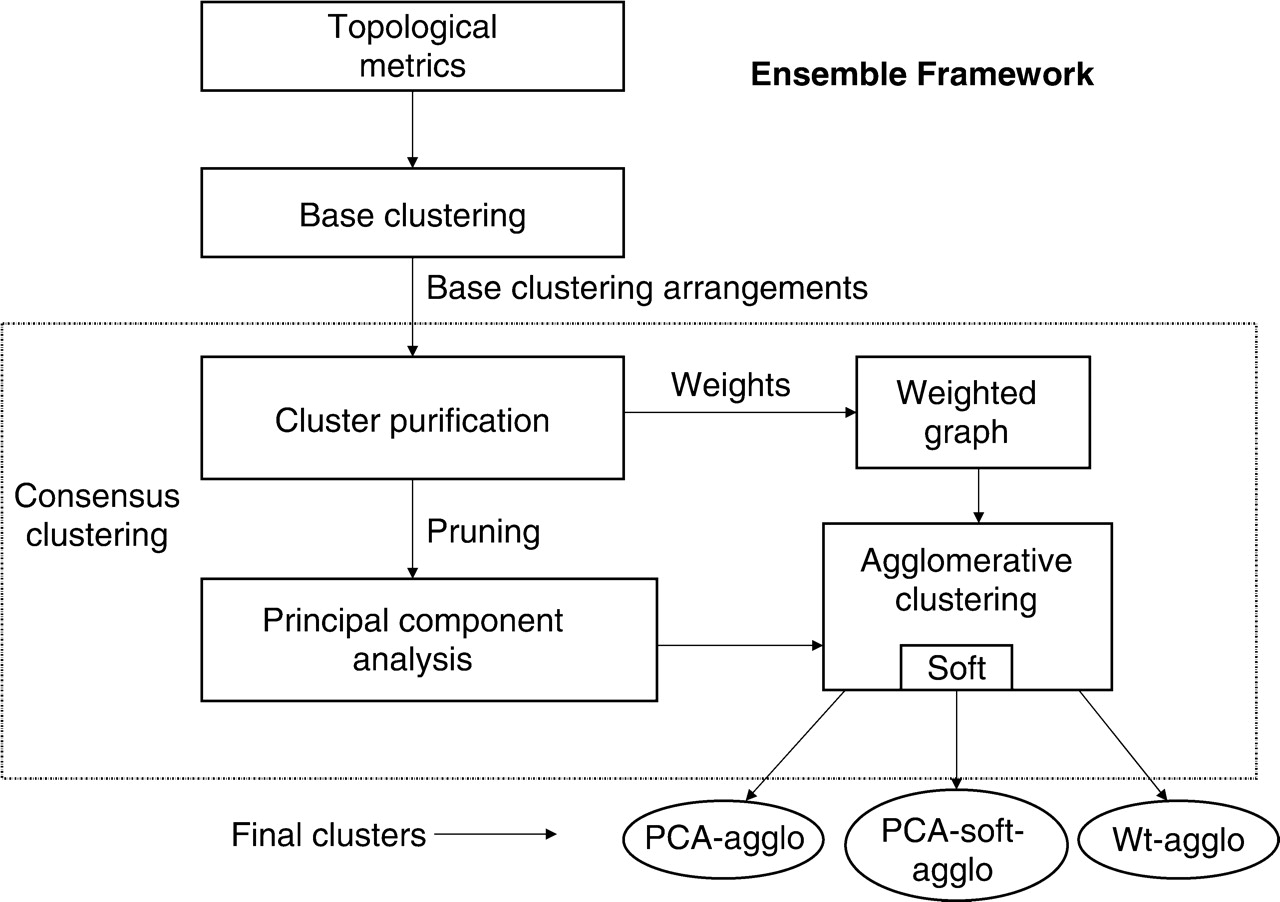
\includegraphics[scale=0.3]{./ensemble_cluster.jpeg}
\caption{Ensemble Framework for Clustering}
\label{fig:ensemble_cluster}
\end{figure}

In Figure \ref{fig:ensemble_cluster}, a flow for the ensemble framework can be seen. In  this figure 
there are two topological similarity metrics that will be used i.e., consensus methods 
and base clustering algorithms. The metrics are used to identify the reliability of PPI 
network interactions. Then based on that eliminate edges that give more false 
positives.\cite{wu_comprehensive_2020} The edge elimination is determined based on the 
weight assigned to edges and that weight is determined by topological features such as 
edge betweenness and clustering coefficient.

Initially, to obtain base clusters three conventional graph clustering algorithms are applied:
\begin{itemize}
    \item \textbf{Direct k-way partitioning} is a clustering solution in which $k$ objects are selected from the data set, these objects act as seed for the $k$ clusters. They are then assigned to each cluster based on the how much similar they are to these clusters. This is continuously refined so that the I2 clustering criterion function could be optimized.
    \item \textbf{Multilevel k-way partitioning} works in three phases, which are coarsening, initial partitioning and refinement. In coarsening, the original graph is divided into smaller graphs. Then in the next phase k-way partitioning of the coarsest graph takes place which satisfies the balance constraints and minimizes the cut value. Allowing for the partitioning to be projected back to the original graph. Finally, refinement reduces the edge-cut while making sure that balance constraints are not affected.  
    \item \textbf{Repeated bisections} is a top-down clustering solution, in which input matrix is clustered into two groups. After that, one of the groups is selected and bisected until the desired number of clusters are found. The clusters are bisected at each point to optimize the I2 clustering criterion function.
\end{itemize}

After getting the base clusters, the next step would be to combine the clusters to get a consensus clustering. To do that, we have to apply a consensus technique which consists of three stages:

\begin{itemize}
    \item \textbf{Cluster Purification}, the objective here is to find clusters that are less consistent with the topology of the original graph. To do that, a reliability measure for each cluster is defined which is based on the topology of proteins in the cluster. Then an intra-cluster distance, i.e., the average shortest path distance between all pair of proteins, is measured for each cluster. The reliability of a cluster is inversely proportional to its intra-cluster distance. A threshold value is then set to prune away weak clusters.
    \item \textbf{Dimensionality Reduction}: Even after pruning, the remaining clusters would still be a lot and the scaling of these clusters to higher dimensional points would likely prove to be inefficient. Which is why the dimensionality reduction would reduce the number of dimensions of cluster-membership matrix without affecting the information needed for clustering. Here, a logistic Principal Component Analysis (PCA) would be used to reduce the dimensions. After this, traditional clustering algorithms can be applied here to get the consensus clustering arrangements. 
    \item In \textbf{Consensus clustering} two consensus clustering algorithms would be applied on the PCA representation obtained from the previous step. The first algorithm, Recursive Bisection algorithm, performs the best of the three base algorithms. Then Agglomerative Hierarchical algorithm, a bottom-up clustering algorithm, assigns each object to its own cluster then continuously merge the pair of clusters until a single or desired number of clusters are obtained.  
\end{itemize}

Now on the acquired clusters there could be a possibility that some proteins are multi-functional. So to account for such cases \textsc{soft consensus clustering} would be applied in the agglomerative hierachical algorithm as there can be some proteins that are part of different clusters.